\documentclass[12pt,letterpaper]{article}

\usepackage{amssymb,amsfonts,amsmath,subfig,chngpage}

\usepackage{times,graphicx,float,bm,adjustbox}

\begin{document}

\title{Supplementary Information}

\date{}

\maketitle

\clearpage

\begin{figure}[t]
\centering
\textbf{Unrotated Solution}\par\medskip
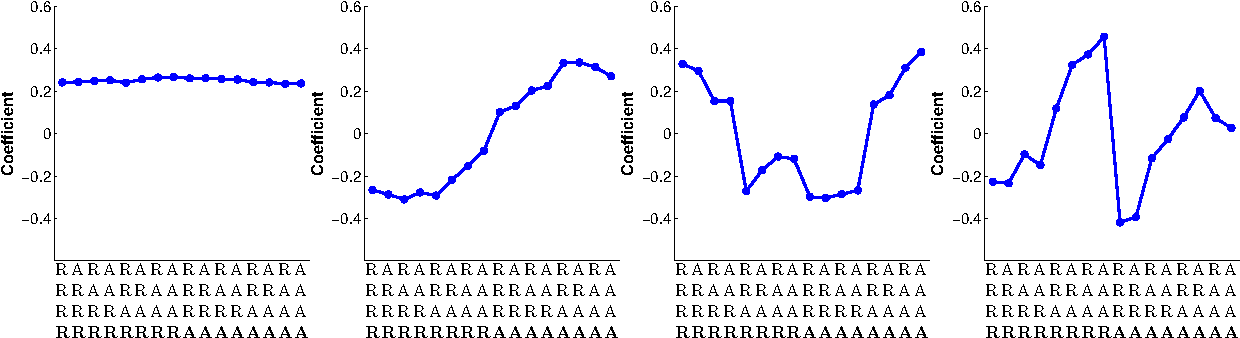
\includegraphics[width=1\textwidth]{unrotated_solution.pdf}
\caption[Unrotated latent structure]{Unrotated latent structure. Coefficient patterns of the four first components extracted with PCA, before rotation. From left to right, components are ordered by amount of variance explained: 78\%, 12\%, 5\% and 1.26\%; variance explained by the remaining components goes 1.03\%, 0.59\%, 0.36\%,...,0.07\%. The first component is clearly interpretable the effect of overall individual mean RT; the second and third components - C2 and C3 - can be interpreted as the effects of the last and second-to-last events respectively; the fourth component exhibits an approximate dependence on the second-to-last independently of the last event, visible as an overall similarity between the left and right halves of the plot.}\label{unrotated_solution}
\end{figure}

\clearpage

%\begin{figure}[T]
%\centering
%\textbf{Subject scores}\par\medskip
%\includegraphics[width=1\textwidth]{subject_scores.pdf}
%\caption{Subject scores.}
%\end{figure}

\begin{figure}[t]
\centering
\begin{tabular}{c}
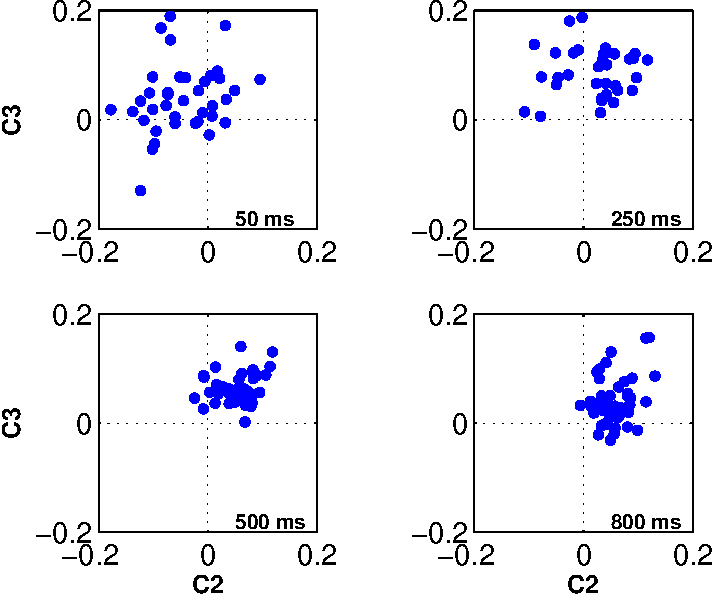
\includegraphics[width=0.33\textwidth]{C2_vs_C3.pdf}\\
a) c12\\
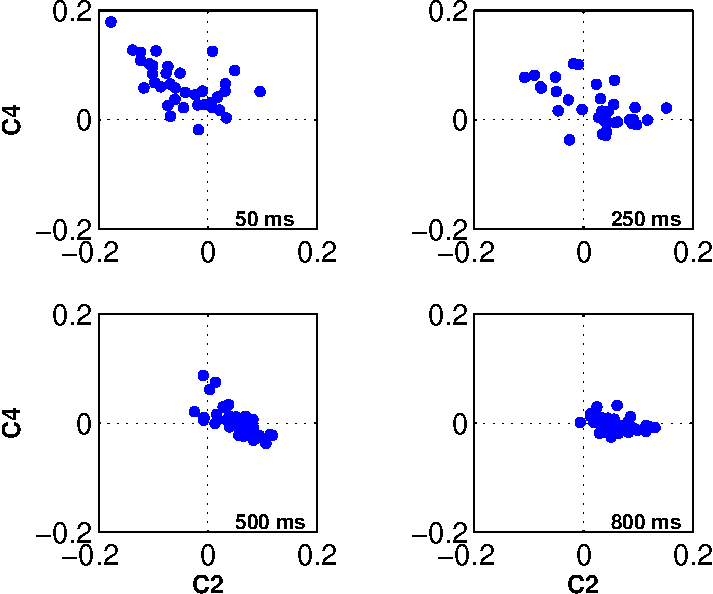
\includegraphics[width=0.33\textwidth]{C2_vs_C4.pdf}\\
b) c24\\
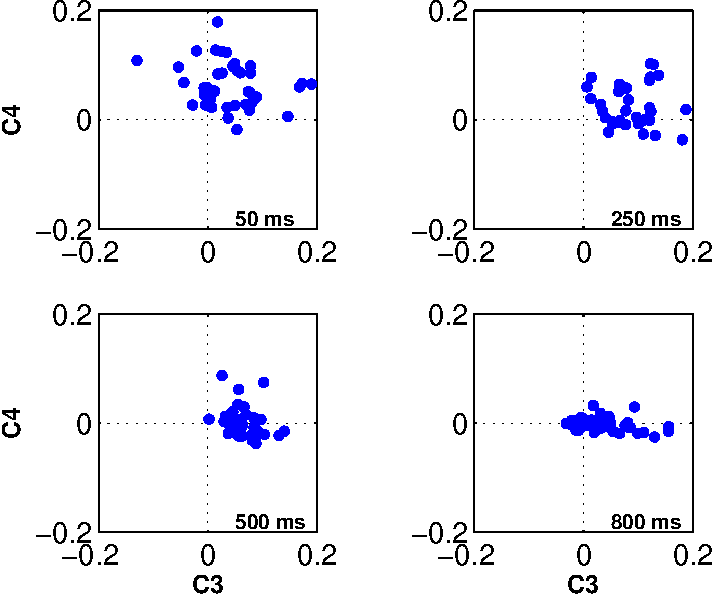
\includegraphics[width=0.33\textwidth]{C3_vs_C4.pdf}\\
c) c34
%\subfloat[C2 vs C3]{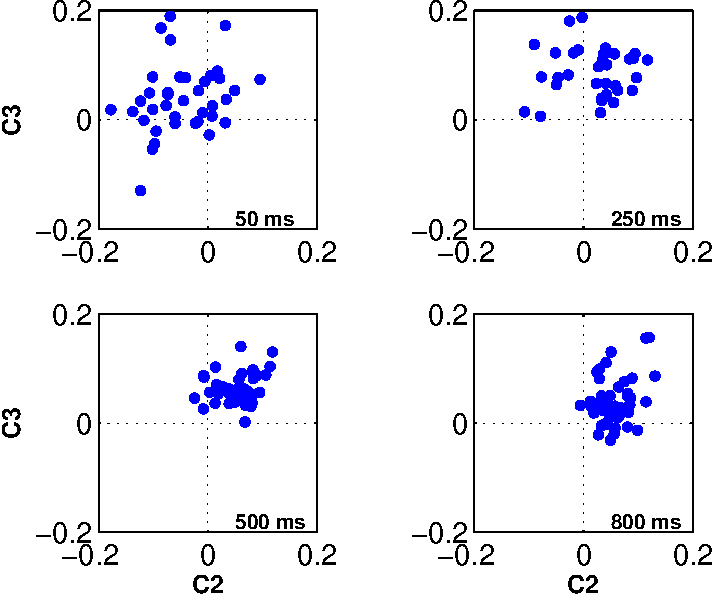
\includegraphics[width=0.33\textwidth]{C2_vs_C3.pdf}\label{c12}}\\
%\subfloat[C2 vs C4]{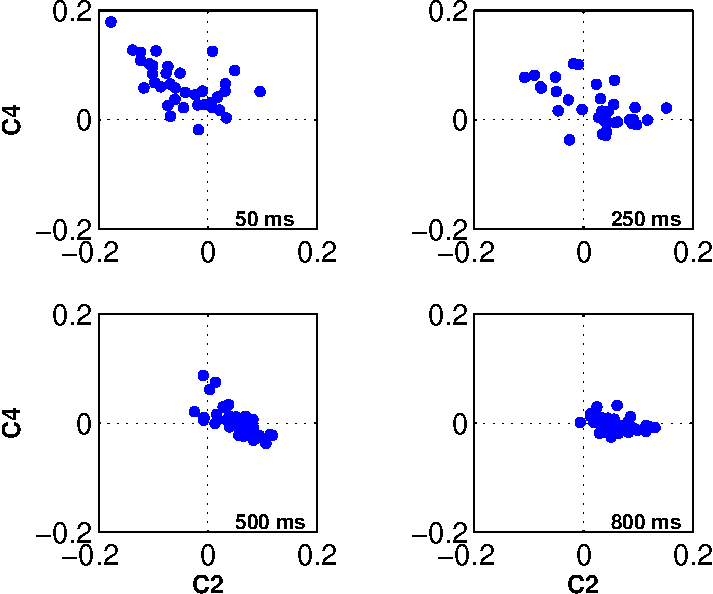
\includegraphics[width=0.33\textwidth]{C2_vs_C4.pdf}\label{c24}}\\
%\subfloat[C3 vs C4]{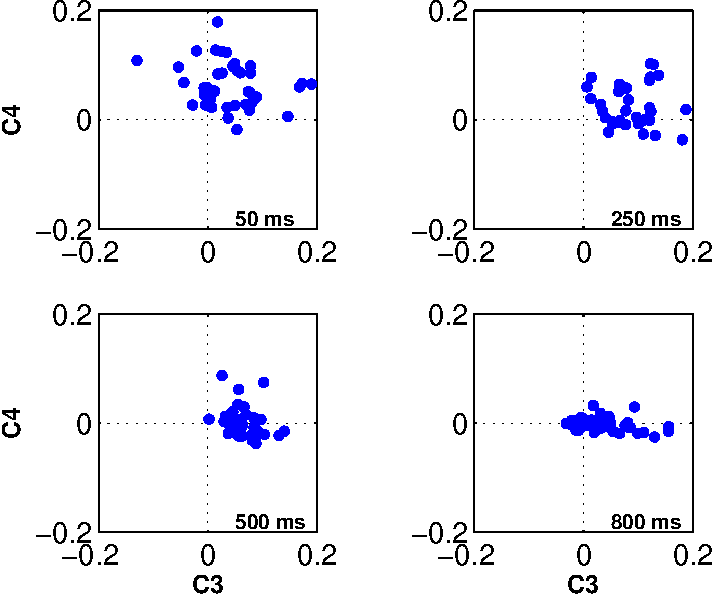
\includegraphics[width=0.33\textwidth]{C3_vs_C4.pdf}\label{c34}}
\end{tabular}
\caption[Individual scores]{Individual scores for all 158 participants on the three latent components related to sequential effects.(a)-(b) panels with scores on one particular component plotted against those on another component. Within each panel, individual RSI subgroups are plotted separately. Details of how the scores were calculated are detailed in the text. Note that the scores were those obtained from the global PCA analysis including all participants. Note that, for a 500 and 800 ms RSI, most subjects have a score on C4 close to zero, reflecting the absence of this component for long RSI values (panels (b) and (c)). In addition, note the correlation between C2 and C4 score for low RSI (middle panel, 50 and 250 ms subgroups). Finally, observe the single subject which exhibits a significantly negative score on both C2 and C3 (top panel, 50 ms subgroup); note that the good qualitative nature of the fit to this subject (not shown) is indicative that these negative scores may not be spurious. In other words, it might be possible - yet rare - to have a negative score on both C2 and C3.}
\end{figure}

\clearpage

\section*{Recalculation of component scores}

Under normal circumstances the PCA model's prediction for the j-th individual is obtained through $\mathbf{x_j} = \bm{\mu} + \sum^N_{i=1} s_i^j \mathbf{C_i}$, where $\mu$ is the grand mean array, $N$ is the number of components retained, $\mathbf{C_i}$ is the coefficient pattern for each component and $s_j^i$ is the the score of subject $j$ on component $i$. If we replace the grand mean with a simple constant, our model becomes $\mathbf{x_j} = b_j + \sum^N_{i=1} s_i^j \mathbf{C_i}$, with $b$ equal to individual overall mean RT. If we further discount the mean RT by subtracting it from each individual, we can set the baseline RT at zero for all subjects, in which case our model further reduces to $\mathbf{x_j} = \sum^N_{i=1} c_i^j \mathbf{V_i}$, where the notation has been changed to highlight the fact that the scores are now linear coefficients and the coefficient patterns simply vectors equal to the coefficient patterns identified with PCA. Individual scores will be estimated by fitting a linear combination of coefficient patterns to each individual's data with the overall mean subtracted. As expected, the linear coefficients thus obtained are almost perfectly correlated to the scores obtained with PCA ($r = 0.92$, $r = 0.97$ and $r = 0.89$ respectively for C2, C3 and C4, $p << 1e-3$ in all cases). It is to these linear coefficients that we refer throughout as individual `scores'.

%Mathematically this is equivalent to forcing the manifold identified with PCA to pass trough the origin, once the main source of variation (individual overall mean RT) has been subtracted away.

\clearpage

\section*{Invariance of latent structure with RSI and Experiment}

\begin{figure}[t]
\centering
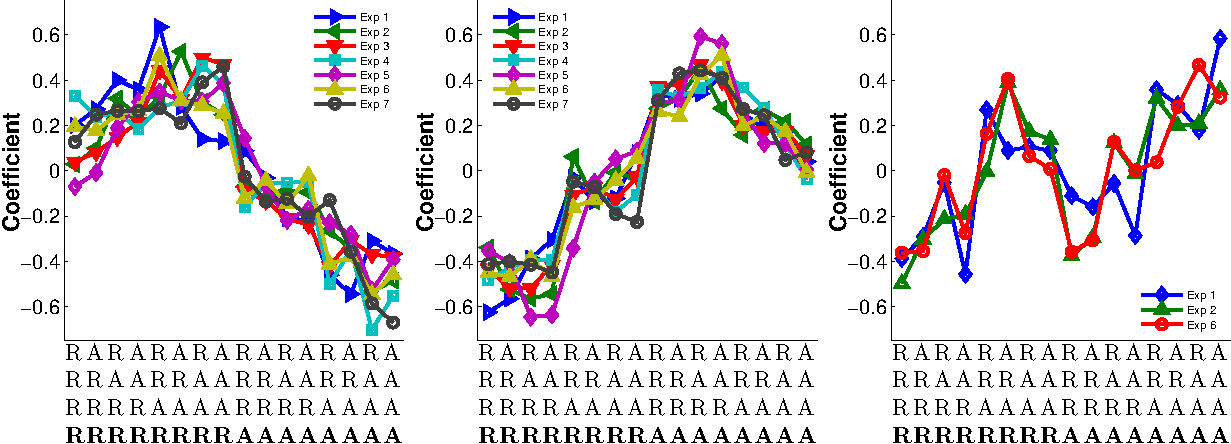
\includegraphics[width=1\textwidth]{components_exp.pdf}
\caption[Latent structure per experiment]{Coefficient patterns obtained by performing a PCA on different subgroups of participants performing different experiments. Plots show, from left to right, C2, C3 and C4. All experiments considered (1 through 7) yielded a C2 and C3 significantly similar to those obtained in the global analysis including all subjects. Only experiments 1, 2 and 6 yielded a C4 significantly similar to the global components. The reason for this is probably the small number of participants in each subgroup together with the fact that C4 explains a relatively small amount of variance. Together, these results clearly indicate that the latent structure obtained with the global analysis is not an artifact of grouping different experiments. }\label{components_exp}
\end{figure}

The non-standard approach of analysing data from multiple experiments together might raise concerns regarding whether the latent structure is constant across conditions. For instance, it would be possible in principle for a component to be present exclusively in one experiment in which case our results would be an artefact of mixing qualitatively different results. In order to dispel these doubts extra care was taken to demonstrate that the latent structure of sequential effects is invariant with respect to both RSI as well as experimental design. This is particularly relevant in the case of different RSI values, given the prevalent view that short and long RSI sequential effects are qualitatively different. In order to evaluate how the latent structure varies, the same analysis which was conducted for all subjects together will be performed in different subgroups separated according to RSI, irrespective of experiment, and according to experiment performed, collapsing across RSI. Different latent structures were obtained, one for each subgroup, and four components were retained each case. It was then necessary to evaluate whether these components were the same as the ones in the global pool of subjects, and this was done with recourse to Tucker index of similarity \cite{Gorsuch83} according to the following procedure: the index was calculated between all putative components of the same type (say C1), one at a time, and the global corresponding component (C1 in this case), and similarly for the remaining three components. The significance of the calculated coefficient values was assessed by holding one vector fixed and randomly permuting the other, allowing a $p$ value to be estimated \cite{Abdi07}. 

\clearpage

\begin{table}[t]
\centering
\begin{adjustbox}{width=1\textwidth}
\begin{tabular}{c|cccccccccccccccc}
Figure & \\
\hline
3 & 32 & 47 & 58 & 65 & 65 & 53 & 64 & 68 & 62 & 62 & 54 & 73 & 56 & 45 & 71 & 55 \\ 
3 & 39 & 46 & 55 & 52 & 83 & 75 & 65 & 53 & 50 & 60 & 53 & 59 & 55 & 49 & 59 & 60 \\ 
3 & 54 & 48 & 68 & 50 & 74 & 80 & 116 & 93 & 50 & 72 & 72 & 76 & 79 & 101 & 97 & 105 \\ 
3 & 31 & 39 & 40 & 52 & 55 & 64 & 76 & 58 & 42 & 36 & 56 & 48 & 68 & 73 & 63 & 61 \\ 
3 & 43 & 37 & 46 & 48 & 38 & 48 & 41 & 50 & 58 & 57 & 52 & 51 & 44 & 36 & 44 & 35 \\ 
3 & 35 & 42 & 43 & 39 & 52 & 61 & 51 & 67 & 50 & 49 & 53 & 44 & 73 & 61 & 61 & 67 \\ \hline
9 & 44 & 46 & 46 & 36 & 39 & 41 & 38 & 35 & 57 & 58 & 78 & 78 & 69 & 32 & 34 & 39 \\ 
9 & 60 & 84 & 86 & 84 & 74 & 90 & 94 & 112 & 68 & 79 & 102 & 102 & 96 & 109 & 101 & 85 \\ 
9 & 27 & 26 & 44 & 45 & 50 & 56 & 39 & 52 & 74 & 55 & 48 & 56 & 52 & 51 & 45 & 48 \\ \hline
10 & 43 & 37 & 53 & 45 & 42 & 52 & 55 & 54 & 60 & 62 & 57 & 58 & 41 & 45 & 52 & 53 \\ 
10 & 68 & 60 & 76 & 72 & 91 & 90 & 98 & 93 & 27 & 49 & 127 & 63 & 156 & 98 & 118 & 112 \\ \hline
11 & 58 & 59 & 82 & 84 & 114 & 150 & 104 & 101 & 43 & 85 & 82 & 96 & 91 & 112 & 112 & 106 \\ 
11 & 45 & 54 & 61 & 66 & 85 & 114 & 76 & 77 & 47 & 50 & 58 & 100 & 69 & 66 & 72 & 70 \\ 
11 & 38 & 49 & 50 & 49 & 62 & 69 & 91 & 92 & 53 & 79 & 78 & 89 & 111 & 118 & 130 & 113 \\ \hline
\end{tabular}
\end{adjustbox}
\caption[]{Standard deviation values for all the individual subjects shown in the main text. Columns are the 16 variables (i.e. sequences) as ordered in the plots throughout. Subjects are ordered from top to bottom on the table as they are shown on the article from left to right.}
\end{table}

\clearpage

\begin{table}[t]
\centering
\begin{adjustbox}{width=1\textwidth}
\begin{tabular}{c|cccccccccccccccc}
Figure & \\
\hline
3 & 153 & 1057 & 652 & 763 & 542 & 1060 & 481 & 71 & 211 & 112 & 95 & 577 & 923 & 723 & 632 & 943 \\ 
3 & 408 & 927 & 1135 & 1011 & 717 & 683 & 536 & 753 & 38 & 392 & 105 & 712 & 569 & 747 & 1173 & 1215 \\ 
3 & 1772 & 906 & 1217 & 497 & 907 & 1371 & 1442 & 912 & 175 & 332 & -10 & 390 & 756 & 467 & 1223 & 1146 \\ 
3 & 420 & 496 & 541 & 978 & 759 & 1036 & 1137 & 500 & 294 & 442 & 948 & 693 & 882 & 561 & 773 & 587 \\ 
3 & 535 & 565 & 501 & 8 & 211 & 217 & 391 & 52 & -111 & 127 & 335 & 510 & 613 & 768 & 1057 & 826 \\ 
3 & 598 & 355 & 580 & 729 & 482 & 745 & 633 & 760 & 549 & 838 & 666 & 546 & 799 & 459 & 715 & 685 \\ \hline
9 & -584 & -400 & 255 & -46 & 860 & 318 & 403 & 552 & 736 & 631 & 1059 & 1110 & 1328 & 67 & 69 & 317 \\ 
9 & 1323 & 948 & 1040 & 627 & 481 & 703 & 734 & 1185 & 858 & 892 & 739 & 466 & 268 & 657 & 698 & 788 \\ 
9 & 563 & 459 & 912 & 669 & 255 & 578 & 526 & 923 & 786 & 381 & 287 & 769 & 302 & 896 & 470 & 571 \\ \hline
10 & 383 & 131 & 537 & 492 & 553 & 655 & 1128 & 85 & 575 & 955 & 657 & 351 & 456 & -24 & 511 & -380 \\ 
10 & 786 & 1007 & 1191 & 653 & 1549 & 909 & -8 & 203 & -19 & -330 & 1081 & 822 & 804 & -15 & 101 & 931 \\ \hline
11 & 786 & 951 & 818 & 961 & 955 & 700 & 1066 & 485 & 458 & 1192 & 913 & 1757 & 725 & 768 & 812 & 1028 \\ 
11 & 395 & 650 & 586 & 605 & 1664 & 986 & 950 & 908 & 823 & 1053 & 971 & 876 & 1241 & 848 & 901 & 741 \\ 
11 & 136 & 604 & 579 & 1022 & 881 & 929 & 934 & 880 & 486 & 522 & 513 & 896 & 587 & 446 & 556 & 705 \\ \hline
\end{tabular}
\end{adjustbox}
\caption[]{Skewness values for all the individual subjects shown in the main text. Columns are the 16 variables (i.e. sequences) as ordered in the plots throughout. Subjects are ordered from top to bottom on the table as they are shown on the article from left to right.}
\end{table}

\clearpage

\begin{table}[t]
\centering
\begin{adjustbox}{width=1\textwidth}
\begin{tabular}{c|cccccccccccccccc}
Figure & \\
\hline
3 & 3206 & 4028 & 2757 & 2630 & 2722 & 4239 & 2673 & 2123 & 2920 & 2564 & 2289 & 2607 & 3336 & 3126 & 2531 & 3312 \\ 
3 & 2604 & 3732 & 4027 & 3697 & 2710 & 2796 & 2677 & 3092 & 2094 & 2523 & 2291 & 3506 & 2592 & 2887 & 3994 & 4079 \\ 
3 & 6648 & 3602 & 4180 & 2379 & 3093 & 5099 & 5267 & 3500 & 2566 & 2614 & 2735 & 3322 & 3507 & 2626 & 4303 & 3803 \\ 
3 & 2807 & 2691 & 2790 & 3230 & 3100 & 3988 & 3841 & 2701 & 2530 & 2448 & 3837 & 3556 & 3218 & 2876 & 4041 & 2933 \\ 
3 & 3450 & 2774 & 2364 & 2819 & 2915 & 2721 & 2342 & 2200 & 1981 & 1857 & 2407 & 2670 & 2621 & 3249 & 3556 & 3434 \\ 
3 & 3012 & 3060 & 3077 & 3527 & 2637 & 3728 & 3107 & 2977 & 3035 & 3379 & 2890 & 2713 & 3071 & 2937 & 3335 & 3321 \\ \hline
9 & 3143 & 2512 & 4403 & 2829 & 3740 & 2489 & 3970 & 2847 & 3102 & 3176 & 3271 & 3433 & 6673 & 3100 & 2603 & 7516 \\ 
9 & 5314 & 2931 & 3801 & 2924 & 2549 & 3549 & 3141 & 3870 & 3470 & 3356 & 2611 & 2634 & 2344 & 2590 & 2553 & 2798 \\ 
9 & 3474 & 3283 & 3484 & 2899 & 2222 & 3479 & 2953 & 3500 & 3499 & 2811 & 2342 & 3509 & 2257 & 4249 & 2916 & 2827 \\ \hline
10 & 2811 & 2967 & 2661 & 2891 & 3323 & 3674 & 5717 & 3002 & 4344 & 6469 & 4623 & 4592 & 4660 & 3566 & 3147 & 4112 \\ 
10 & 2475 & 2914 & 4748 & 2270 & 4695 & 3401 & 2142 & 2125 & 1867 & 2622 & 4696 & 2409 & 3826 & 3253 & 2495 & 4720 \\ \hline
11 & 3251 & 3516 & 2800 & 3628 & 3010 & 2537 & 3219 & 2556 & 2661 & 3903 & 3205 & 6894 & 2651 & 2866 & 3087 & 3719 \\ 
11 & 2317 & 2664 & 2861 & 2917 & 6067 & 3065 & 3215 & 3421 & 3947 & 4572 & 3634 & 2920 & 4436 & 3823 & 4066 & 2903 \\ 
11 & 3092 & 3995 & 3708 & 4449 & 4519 & 4199 & 3374 & 3000 & 2328 & 2597 & 2805 & 3189 & 2805 & 2477 & 2547 & 3053 \\ \hline
\end{tabular}
\end{adjustbox}
\caption[]{Kurtosis values for all the individual subjects shown in the main text. Columns are the 16 variables (i.e. sequences) as ordered in the plots throughout. Subjects are ordered from top to bottom on the table as they are shown on the article from left to right.}
\end{table}

\clearpage

\begin{table}[t]
\centering
\begin{adjustbox}{width=1\textwidth}
\begin{tabular}{c|cccccccccccccccc}
Figure & \\
\hline
3 & 44 & 47 & 54 & 55 & 69 & 71 & 73 & 72 & 63 & 65 & 72 & 70 & 85 & 89 & 81 & 74 \\ \hline
6 & 84 & 85 & 86 & 81 & 90 & 112 & 100 & 104 & 67 & 75 & 89 & 100 & 113 & 134 & 147 & 145 \\ 
6 & 64 & 63 & 68 & 69 & 72 & 83 & 79 & 83 & 70 & 74 & 89 & 86 & 99 & 107 & 105 & 102 \\ 
6 & 56 & 62 & 64 & 67 & 72 & 76 & 76 & 78 & 79 & 80 & 82 & 81 & 85 & 82 & 83 & 79 \\ 
6 & 55 & 56 & 61 & 62 & 68 & 71 & 69 & 69 & 78 & 78 & 82 & 78 & 78 & 77 & 76 & 71 \\ 
\end{tabular}
\end{adjustbox}
\caption[]{Standard deviation values for all the groups of subjects shown in the main text. Columns are the 16 variables (i.e. sequences) as ordered in the plots throughout. Groups of subjects are ordered from top to bottom on the table as they are shown on the article from left to right.}
\end{table}

\clearpage

\begin{table}[t]
\centering
\begin{adjustbox}{width=1\textwidth}
\begin{tabular}{c|cccccccccccccccc}
Figure & \\
\hline
3 & 685 & 627 & 673 & 744 & 742 & 870 & 806 & 582 & 316 & 444 & 424 & 427 & 566 & 594 & 609 & 717 \\ \hline
6 & 1880 & 1889 & 1204 & 1141 & 1191 & 1806 & 1802 & 854 & 1189 & 1341 & 1339 & 1368 & 1387 & 1506 & 1705 & 1960 \\ 
6 & -106 & -120 & 260 & 280 & 447 & 1006 & 882 & 848 & 559 & 459 & 790 & 523 & 853 & 892 & 1116 & 1178 \\ 
6 & 889 & 976 & 967 & 990 & 932 & 981 & 1314 & 1307 & 670 & 802 & 872 & 822 & 843 & 1030 & 1050 & 1339 \\ 
6 & 523 & 596 & 975 & 1027 & 1128 & 1106 & 1549 & 919 & 954 & 947 & 1221 & 989 & 1080 & 1303 & 1343 & 955 \\ 
\end{tabular}
\end{adjustbox}
\caption[]{Skewness values for all the groups of subjects shown in the main text. Columns are the 16 variables (i.e. sequences) as ordered in the plots throughout. Groups of subjects are ordered from top to bottom on the table as they are shown on the article from left to right.}
\end{table}

\clearpage

\begin{table}[t]
\centering
\begin{adjustbox}{width=1\textwidth}
\begin{tabular}{c|cccccccccccccccc}
Figure & \\
\hline
3 & 3667 & 3268 & 3313 & 3212 & 3024 & 3619 & 3290 & 2965 & 2798 & 2951 & 2771 & 2927 & 2978 & 2880 & 3383 & 3254 \\ \hline
6 & 11223 & 12391 & 6620 & 6445 & 6708 & 8490 & 10261 & 4892 & 5371 & 5954 & 5553 & 6111 & 5740 & 6337 & 7567 & 8749 \\ 
6 & 4231 & 4138 & 4614 & 4217 & 4370 & 5552 & 5100 & 4381 & 3233 & 3052 & 4556 & 3130 & 3862 & 3831 & 4711 & 5058 \\ 
6 & 5490 & 5418 & 5179 & 5206 & 4223 & 4721 & 6686 & 6326 & 3256 & 3576 & 3903 & 3802 & 3570 & 4202 & 4254 & 5428 \\ 
6 & 4070 & 6173 & 5051 & 5390 & 5086 & 5093 & 8515 & 4540 & 4107 & 4219 & 5190 & 4225 & 4492 & 5946 & 5656 & 4375 \\ 
\end{tabular}
\end{adjustbox}
\caption[]{Kurtosis values for all the groups of subjects shown in the main text. Columns are the 16 variables (i.e. sequences) as ordered in the plots throughout. Groups of subjects are ordered from top to bottom on the table as they are shown on the article from left to right.}
\end{table}

\clearpage


\begin{table}[t]
\centering
\begin{tabular}{ccc}
Figure &Mean & Stand. dev.\\ \hline
3 & 0.94 & 0.02 \\ 
3 & 0.92 & 0.04 \\ 
3 & 0.92 & 0.03 \\ 
3 & 0.91 & 0.04 \\ 
3 & 0.91 & 0.03 \\ 
3 & 0.94 & 0.03 \\ \hline
9 & 0.95 & 0.02 \\ 
9 & 0.90 & 0.04 \\ 
9 & 0.93 & 0.03 \\ \hline
10 & 0.83 & 0.06 \\ 
10 & 0.92 & 0.04 \\ \hline
11 & 0.88 & 0.05 \\ 
11 & 0.90 & 0.04 \\ 
11 & 0.95 & 0.02 \\ \hline
\end{tabular}
\caption[]{Reliability of the results of all individuals shown in the main text. Subjects are ordered from top to bottom on the table as they are shown on the article from left to right. Split half reliability was used: data was was randomly split into two halves resulting in two different sequential effects patterns and the correlation coefficient between the two was calculated. Values shown are the mean and standard deviation of the correlation coefficients obtained from 100 iterations of the split-half procedure.}
\end{table}

\clearpage

\begin{table}[t]
\centering
\begin{tabular}{ccc}
Figure & Mean & Stand. dev.\\ \hline
3 & 0.9720 & 0.0109 \\ \hline
6 & 0.9946 & 0.0024 \\ 
6 & 0.9942 & 0.0025 \\ 
6 & 0.9914 & 0.0036 \\ 
6 & 0.9910 & 0.0033 \\ 
\end{tabular}
\caption[]{Reliability of the results of all groups of subjects shown in the main text. Subjects are ordered from top to bottom on the table as they are shown on the article from left to right. Split half reliability was used: data was was randomly split into two halves resulting in two different sequential effects patterns and the correlation coefficient between the two was calculated. Values shown are the mean and standard deviation of the correlation coefficients obtained from 100 iterations of the split-half procedure.}
\end{table}

\clearpage

\bibliographystyle{apacite}

\begin{thebibliography}{}

\bibitem{Abdi07}
Herv{\'e} Abdi.
\newblock Rv coefficient and congruence coefficient.
\newblock {\em Encyclopedia of measurement and statistics}, pages 849--853,
  2007.

%\bibitem{Cattell65}
%Raymond Cattell.
%\newblock {The Scree Test For The Number Of Factors}.
%\newblock {\em Multivariate Behavioral Research}, 1:245--276, 1966.
%
%\bibitem{Cho02}
%Raymond~Y. Cho, Leigh~E. Nystrom, Eric~T. Brown, Andrew~D. Jones, Todd~S.
%  Braver, Philip~J. Holmes, and Jonathan~D. Cohen.
%\newblock Mechanisms underlying dependencies of performance on stimulus history
%  in a two-alternative forced-choice task.
%\newblock {\em Cognitive, Affective, \& Behavioral Neuroscience},
%  4(2):283--299, 2002.
%
%\bibitem{Gokaydin11}
%D.~Gokaydin, Anna Ma-Wyatt, D.~J. Navarro, and Amy Perfors.
%\newblock Humans use different statistics for sequence analysis depending on
%  the task.
%\newblock {\em Proceedings of the 33rd Annual Conference of the Cognitive
%  Science Society}, pages 543--548, 2011.
%
\bibitem{Gorsuch83}
Richard~L Gorsuch.
\newblock {\em Factor analysis}.
\newblock L. Erlbaum Associates, Hillsdale, {N.J.}, 1983.
%
%\bibitem{Horn65}
%John Horn.
%\newblock A rationale and test for the number of factors in factor analysis.
%\newblock {\em Psychometrika}, 30(2):179--185, 1965.
%
%\bibitem{Jentzsch02}
%Ines Jentzsch and Werner Sommer.
%\newblock Functional localization and mechanisms of sequential effects in
%  serial reaction time tasks.
%\newblock {\em Perception \& psychophysics}, 64(7):1169--1188, 2002.
%
%\bibitem{Joreskog71}
%K.~Joreskog.
%\newblock Simultaneous factor analysis in several populations.
%\newblock {\em Psychometrika}, 36(4):409--426, 1971.
%
%\bibitem{Soetens85}
%E.~Soetens, L.C. Boer, and J.E. Hueting.
%\newblock Expectancy or automatic facilitation? separating sequential effects
%  in two-choice reaction time.
%\newblock {\em Journal of Experimental Psychology: Human Perception and
%  Performance}, 11(5):598--616, 1985.

\end{thebibliography}

\end{document}

